\chapter{Experiment setup}
\indent
    Experiment setup is listed in this chapter including 3 parts, 
    dataset, models, and activation functions.

\section{Dataset}
\indent
    BCI Competition III - IIIb dataset includes cued motor imagery with online feedback, which is non-stationary classifier,
    with 2 classes, left hand and right hand, from 3 subjects, 2 classes and 2 bipolar EEG channels (See Figure \ref{dataset}).\\
    The dataset is split into training and testing set, and the input data shape is \code{[B, 1, 2, 750]}, and output is \code{[B, 2]}, 
    where \code{B} represents batch size and the third dimension indicates 2 channels (See Figure \ref{dataset-channel}).

    \begin{figure}[H]
		\centering
		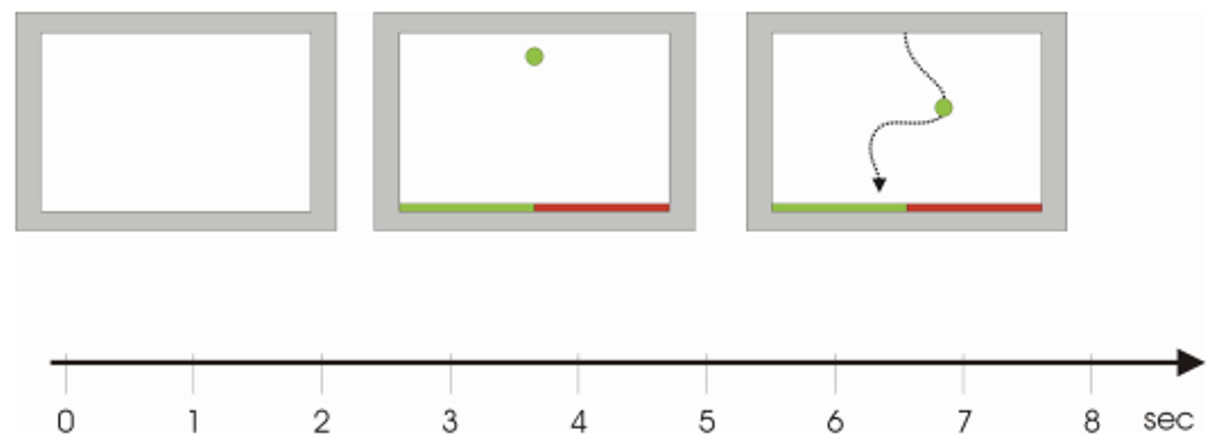
\includegraphics[scale=0.5]{img/dataset.png}
		\caption{BCI Competition III - IIIb dataset.}
		\label{dataset}
	\end{figure}
    \begin{figure}[H]
		\centering
		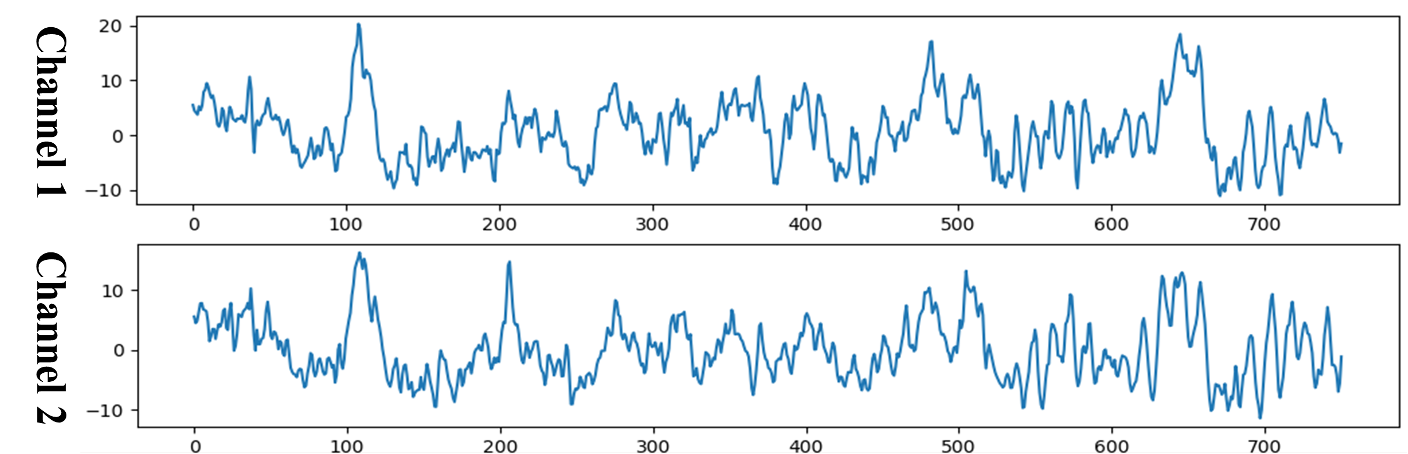
\includegraphics[scale=0.5]{img/dataset_channel.png}
		\caption{2 channels of BCI Competition III - IIIb dataset.}
		\label{dataset-channel}
	\end{figure}

\section{Models}
\indent
    Models details are listed in this section including 2 parts,
    EEGNet and DeepConvNet.

\subsection{EEGNet}
\indent
	EEGNet is compounded of 3 different 2D convolution blocks, 
	normal, depthwise, and separable 2D convolution blocks, and
	the last layer of this model is a linear layer (See Figure \ref{eegnet}). 
	Details are in Listing \ref{eegnet-code}.

	\begin{figure}[H]
		\centering
		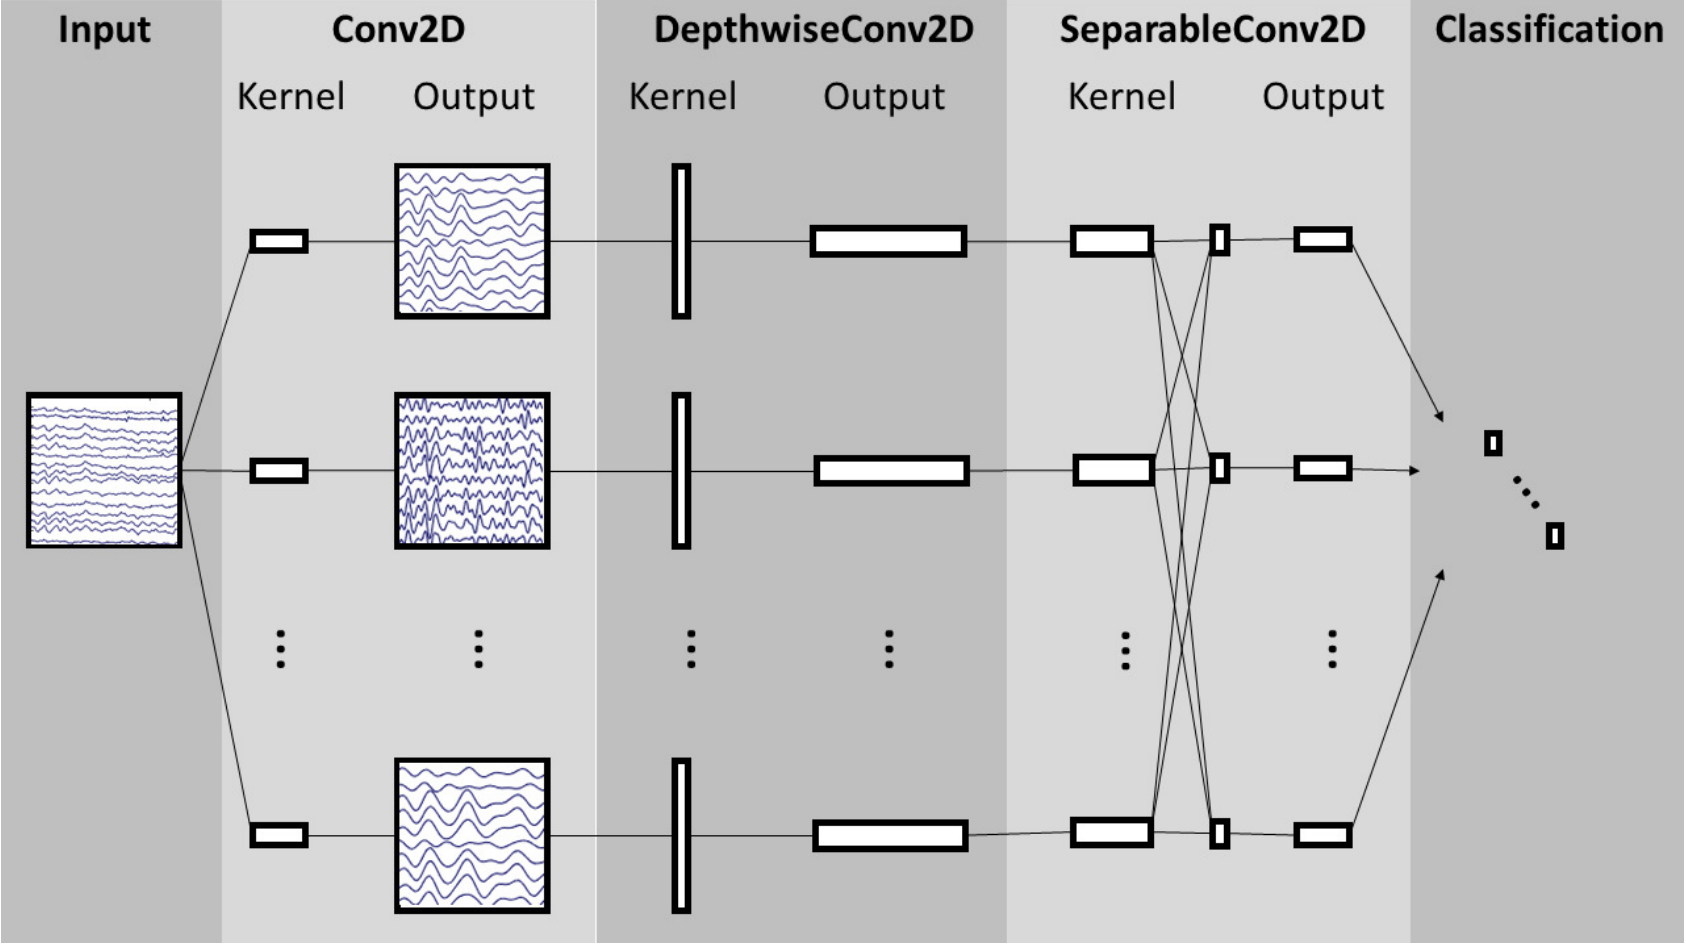
\includegraphics[scale=0.5]{img/eegnet.png}
		\caption{Architecture of EEGNet.}
		\label{eegnet}
	\end{figure}
\pagebreak
\begin{lstlisting}[language=Python, caption={Python code of EEGNet.}, label={eegnet-code}]
self.conv_2d = nn.Sequential(
	nn.Conv2d(
		in_channels=1,
		out_channels=16,
		kernel_size=(1, 51),
		stride=(1, 1),
		padding=(0, 25),
		bias=False
	),
	nn.BatchNorm2d(16)
)
self.depthwise_conv = nn.Sequential(
	nn.Conv2d(
		in_channels=16,
		out_channels=32,
		kernel_size=(2, 1),
		stride=(1, 1),
		groups=16,
		bias=False
	),
	nn.BatchNorm2d(32),
	self.act,
	nn.AvgPool2d(kernel_size=(1, 4), stride=(1, 4), padding=0),
	nn.Dropout(p=dropout)
)
self.separable_conv = nn.Sequential(
	nn.Conv2d(
		in_channels=32,
		out_channels=32,
		kernel_size=(1, 15),
		stride=(1, 1),
		padding=(0, 7),
		bias=False
	),
	nn.BatchNorm2d(32),
	self.act,
	nn.AvgPool2d(kernel_size=(1, 8), stride=(1, 8), padding=0),
	nn.Dropout(p=dropout)
)
self.linear = nn.Sequential(
	nn.Flatten(),
	nn.Linear(in_features=736, out_features=2, bias=True)
)\end{lstlisting}
		
\subsection{DeepConvNet}
\indent
	DeepConvNet is compounded of multiple convolution blocks, and
	the number of channels starts from 1 to 25, then 50, 100, and finally 200.
	The last layer of this model is also a linear layer (See Figure \ref{deepconvnet}). 
	Details are in Listing \ref{deepconvnet-code}.

	\begin{figure}[H]
		\centering
		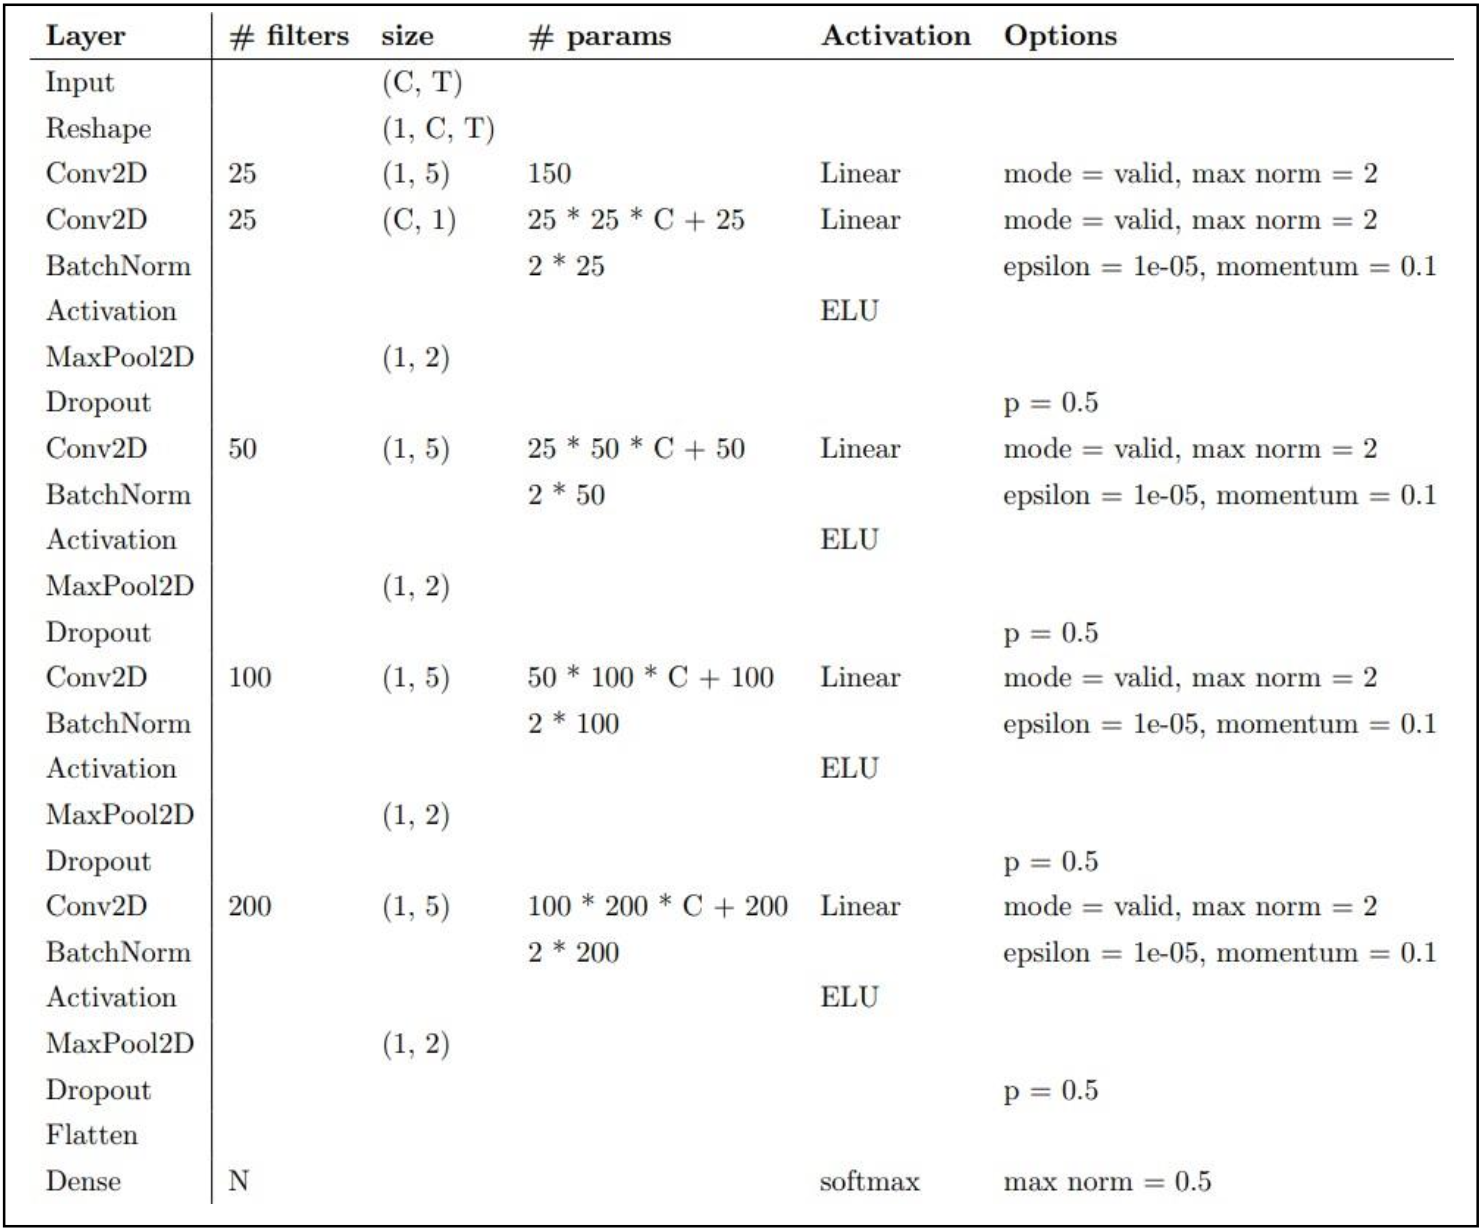
\includegraphics[scale=0.5]{img/deepconvnet.png}
		\caption{Architecture of DeepConvNet.}
		\label{deepconvnet}
	\end{figure}
\begin{lstlisting}[language=Python, caption={Python code of DeepConvNet.}, label={deepconvnet-code}]
self.first_conv = nn.Sequential(
	nn.Conv2d(
		in_channels=1,
		out_channels=25,
		kernel_size=(1, 5),
		bias=False
	),
	nn.Conv2d(
		in_channels=25,
		out_channels=25,
		kernel_size=(2, 1),
		bias=False
	),
	nn.BatchNorm2d(25),
	self.act,
	nn.MaxPool2d(kernel_size=(1, 2)),
	nn.Dropout(p=dropout)
)
layers = [25, 50, 100, 200]
self.convs = nn.ModuleList([
	nn.Sequential(
		nn.Conv2d(
			in_channels=layers[i],
			out_channels=layers[i + 1],
			kernel_size=(1, 5),
			bias=False
		),
		nn.BatchNorm2d(layers[i + 1]),
		self.act,
		nn.MaxPool2d(kernel_size=(1, 2)),
		nn.Dropout(p=dropout))
	for i in range(len(layers) - 1)
])
convs_output_size = 373
flatten_size = 200 * reduce(lambda x, _: round((x - 4) / 2), layers[: -1], convs_output_size) # 8600.
self.linear = nn.Sequential(
	nn.Flatten(),
	nn.Linear(in_features=flatten_size, out_features=2, bias=True)
)
\end{lstlisting}

\section{Activation functions}
\indent
    In this task, 3 activation functions, i.e., \code{ReLU}, \code{LeakyReLU}, and \code{ELU}, 
    are used to compare performance of different activation functions.

\subsection{ReLU}
\indent
    \code{ReLU} clips all negative values and returns 0, and positive values remain the same  (See Figure \ref{relu}). 
    It's one of the mostly used activation functions, and the gradient computation cost is low during backpropagation step.
    Disadvantage is positive values may be infinite and neurons which have negative values may not update.

    \begin{figure}[H]
		\centering
		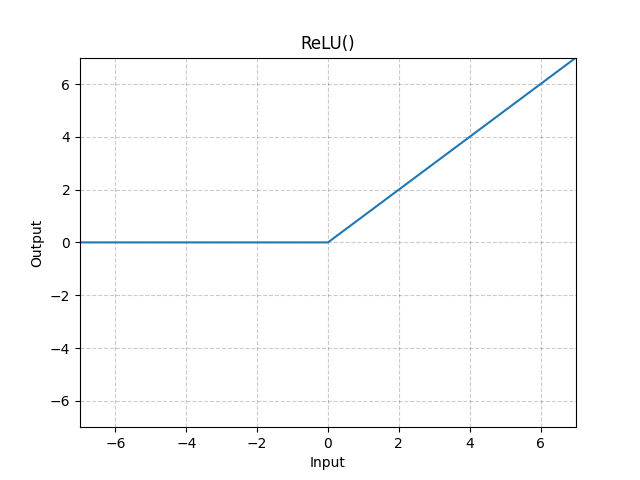
\includegraphics[scale=0.5]{img/relu.png}
		\caption{Illustration of ReLU activation function.}
		\label{relu}
	\end{figure}

\subsection{LeakyReLU}
\indent
    \code{LeakyReLU} is similar to \code{ReLU}, but the negative values backpropagate partially (See Figure \ref{leaky-relu}).

    \begin{figure}[H]
		\centering
		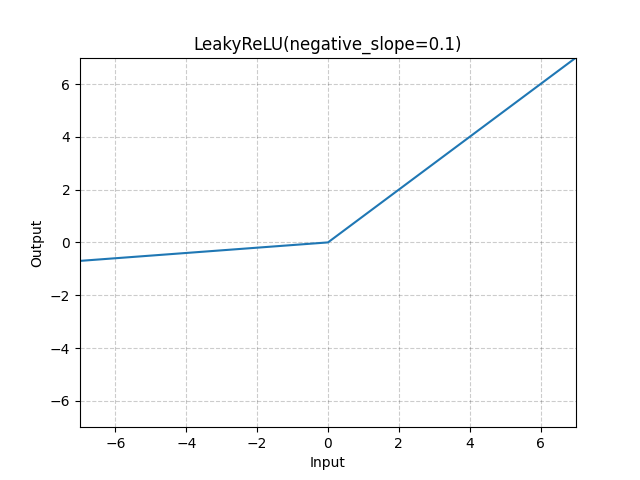
\includegraphics[scale=0.5]{img/leaky-relu.png}
		\caption{Illustration of LeakyReLU activation function.}
		\label{leaky-relu}
	\end{figure}

\subsection{ELU}
\indent
    \code{ELU} is similar to \code{LeakyReLU}, but the negative values returns are smoothed due to the exponential computation (See Figure \ref{elu}).

    \begin{figure}[H]
		\centering
		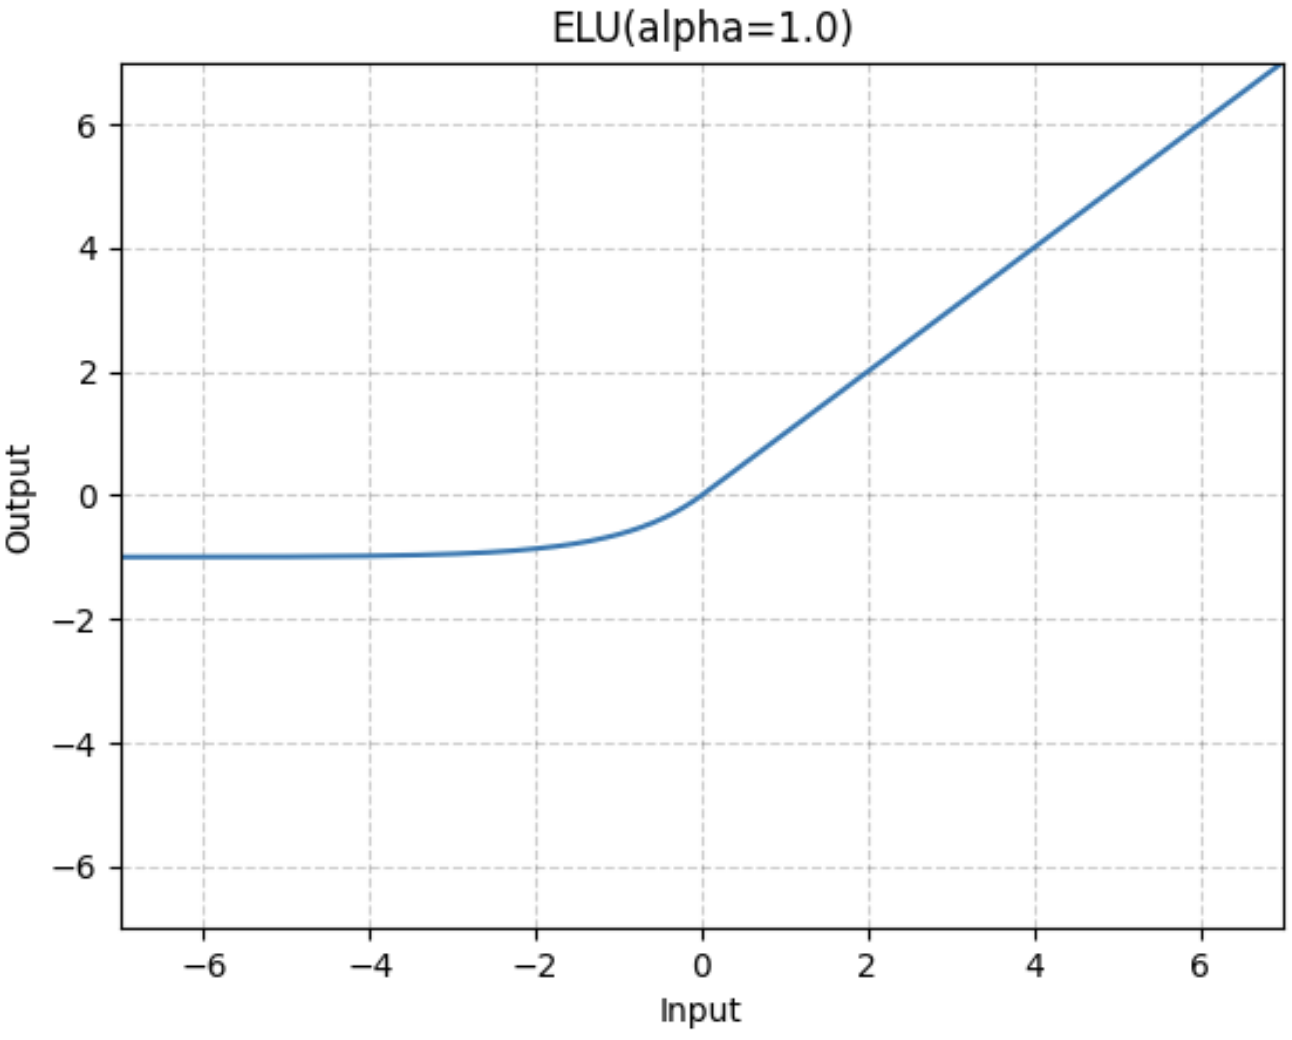
\includegraphics[scale=0.3]{img/elu.png}
		\caption{Illustration of ELU activation function.}
		\label{elu}
	\end{figure}
